\mychapter{Modelling}{Modelling}{}
\label{chap:modelling}

\mysection{Introduction}{Introduction}
\label{sec:modintro}

To accurately describe the full pose of a satellite using an onboard imaging system, a comprehensive mathematical model 
of the spacecraft must be established. This chapter presents the fundamental modeling framework required for vision-based 
satellite pose estimation. The chapter begins by defining the core problem and establishing the system requirements for satellite 
pose determination. Subsequently, the kinematic and dynamic equations governing satellite motion are derived, providing the mathematical 
foundation for state propagation. The various reference frames utilized throughout this work are systematically 
defined, including the transformations necessary to relate measurements and states across different coordinate systems.
Additionally, this chapter presents the mathematical models for the accompanying sensors integrated within the pose estimation system. 
These sensor models are essential for the multi-sensor fusion approach employed in the Extended Kalman Filter implementation presented in later chapters.


%=============================================================================================================================================================================


\mysection{Rigid Body Mechanics}{Rigid Body Mechanics}
\label{sec:modrigid}

\mysubsection{Kinematics}{Kinematics}
\label{sec:kinematics}

The pose of a rigid body within a reference frame encompasses both its spatial position and angular orientation. The 
attitude describes the rotational relationship between the body-fixed coordinate system and a known reference coordinate system. 
This rotational relationship is typically expressed through a rotation matrix, commonly known as a direction cosine matrix (DCM).\cite{Jongh}\cite{Korf}\cite{Jordaan}\cite{Diebel},
Elementary rotations around individual coordinate axes are termed coordinate rotations. The fundamental coordinate rotations about 
the x-, y-, and z-axes, characterized by rotation angles $\phi$, $\theta$, and $\psi$ respectively, can be mathematically expressed as

\begin{equation}
    R_x(\phi) = \begin{bmatrix} 
        1 & 0 & 0 \\
        0 & \cos(\phi) & \sin(\phi) \\
        0 & -\sin(\phi) & \cos(\phi)
    \end{bmatrix}
    \label{Eq:3.1}
\end{equation}

\begin{equation}
    R_y(\theta) = \begin{bmatrix} 
        \cos(\theta) & 0 & -\sin(\theta) \\
        0 & 1 & 0 \\
        \sin(\theta) & 0  & \cos(\theta)
    \end{bmatrix}
    \label{Eq:3.2}
\end{equation}

\begin{equation}
    R_z(\psi) = \begin{bmatrix} 
        \cos(\psi) & \sin(\psi) & 0 \\
        -\sin(\psi) & \cos(\psi) & 0 \\
        0 & 0 & 1
    \end{bmatrix}
    \label{Eq:3.3}
\end{equation}

\noindent Any rotation in 3D space can be described by three coordinate rotations. The DCM describing the rotation from 
the orbital reference frame $\mathcal{O}$ to the body reference frame $\mathcal{B}$, $\mathbf{A}_{\mathcal{O}}^{\mathcal{B}}$, 
can be represented by three Eular angles. Each of the angles corresponds to one coordinate rotation. The order
of the Eular 1-2-3 or a Roll, Ptich, Yaw rotation, shown in Figure 3.5, is expressed as

\begin{equation}
    \boldsymbol{A}_{\mathcal{O}}^{\mathcal{B}} = R_x(\phi)R_y(\theta)R_z(\psi)
    \label{Eq:3.4}
\end{equation}

\begin{equation}
    \begin{bmatrix}
        a_{1,1} & a_{1,2} & a_{1,3}\\
        a_{2,1} & a_{2,2} & a_{2,3}\\
        a_{3,1} & a_{3,2} & a_{3,3}\\
    \end{bmatrix}
\end{equation}

\begin{equation}
    \begin{bmatrix}
        C\theta C\psi & C\theta S\psi &  -S\theta\\
        S\phi S\theta C\psi - C\phi S\psi & S\phi S\theta S\psi + C\phi C\psi & S\phi C\theta\\
        C\phi S\theta C\psi + S\phi S\psi &  C\phi S\theta S\psi - S\phi C\psi & C\phi C\theta
    \end{bmatrix}
\end{equation}

\noindent Where S is the sine function and C is the cosine function. The Eular angles are calculated as follows

\begin{equation}
    \phi = \arctan2\left(\frac{a_{2,3}}{a_{3,3}}\right)
\end{equation}

\begin{equation}
    \theta = \arctan2\left(\frac{-a_{1,3}}{\sqrt{a_{1,1}^2} + \sqrt{a_{1,2}^2}}\right)
\end{equation}

\begin{equation}
    \psi = \arctan2\left(\frac{a_{1,2}}{a_{1,1}}\right)
\end{equation}

\begin{figure}[H]
    \centering
    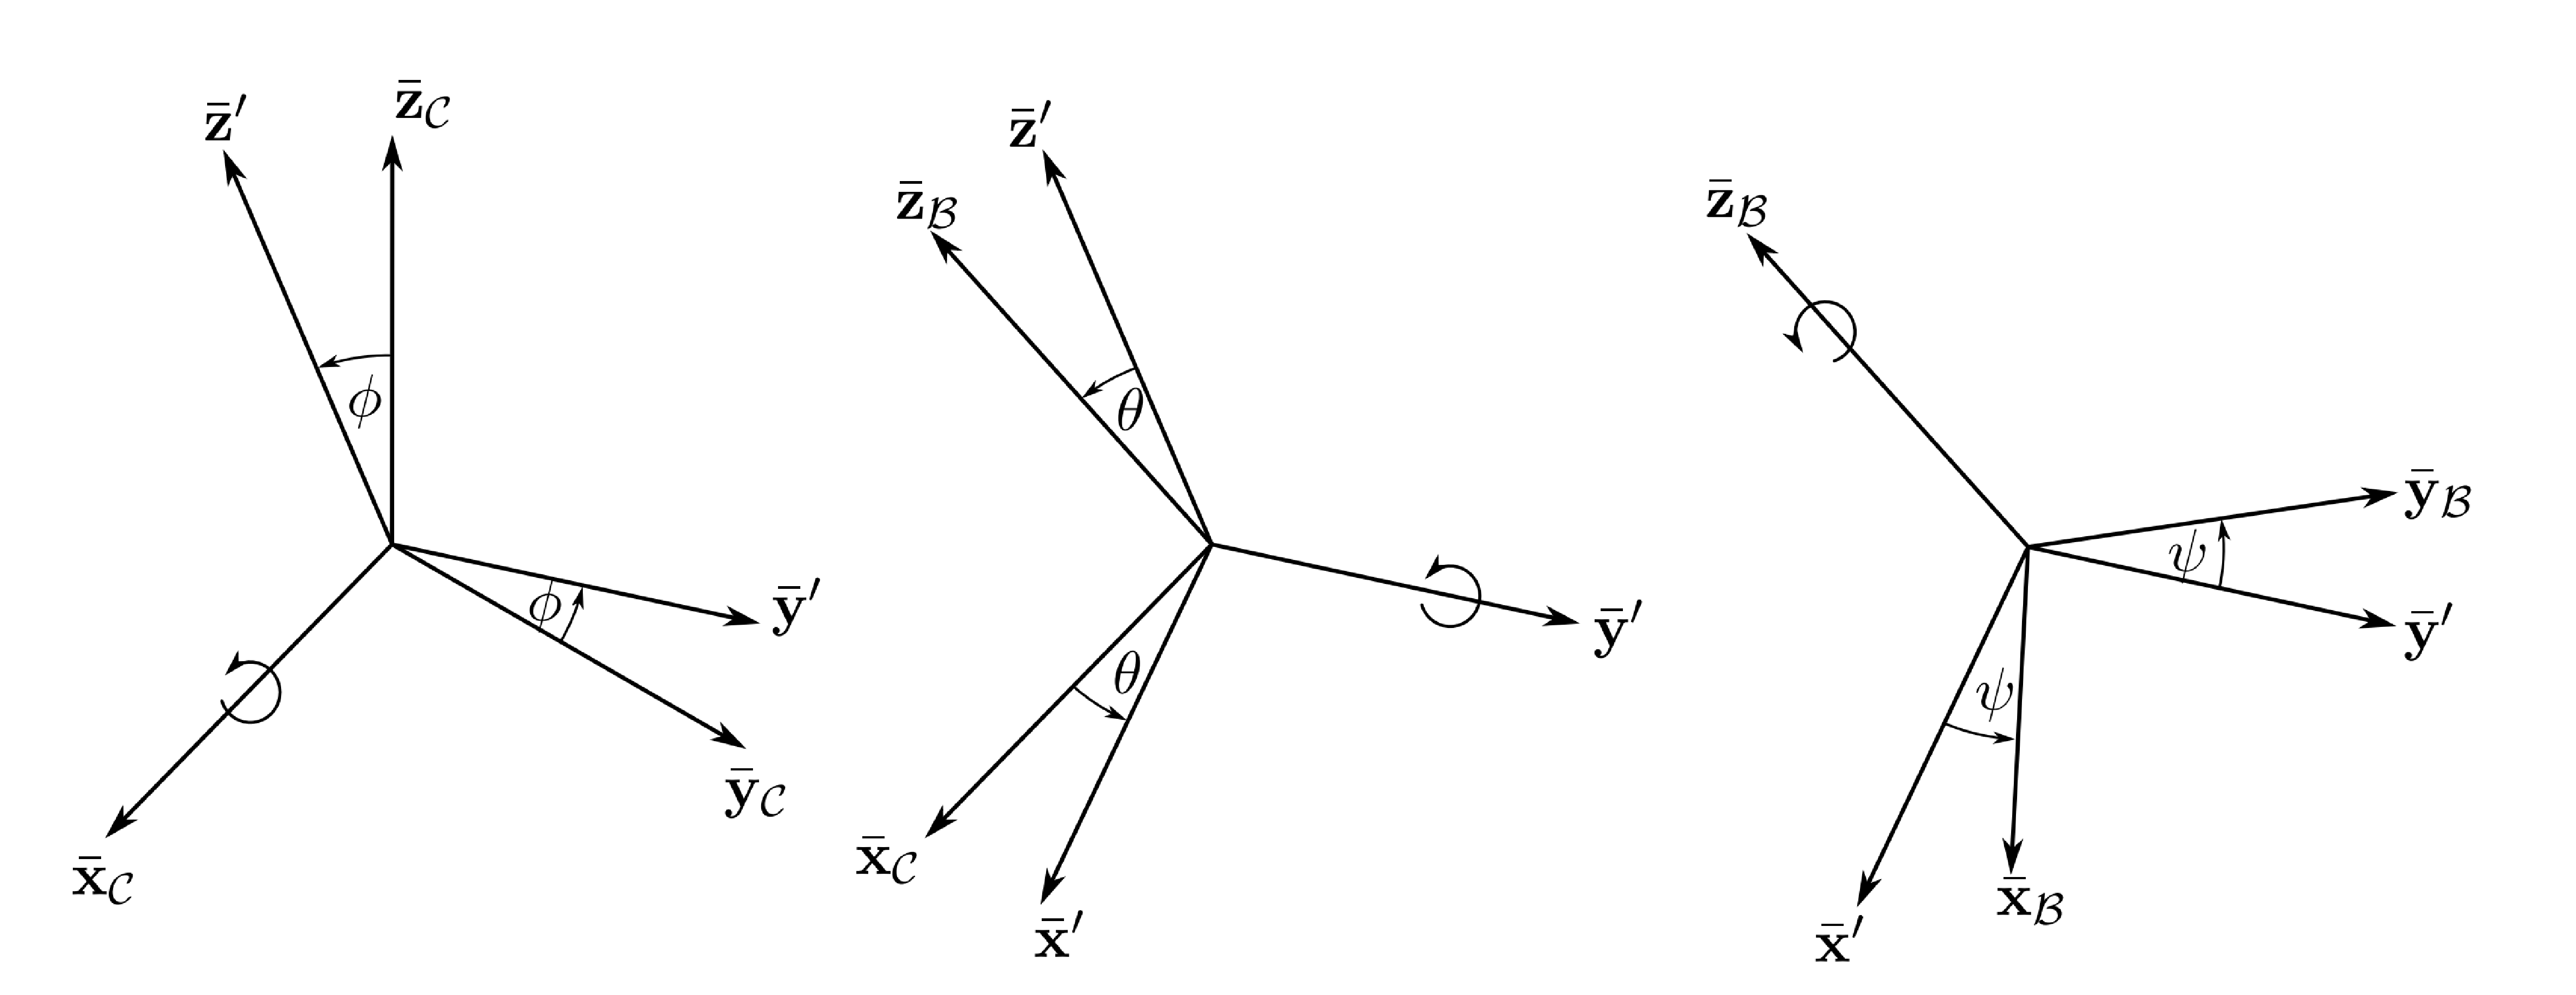
\includegraphics[width=\linewidth]{figures/modelling/213 Eular Rotation.pdf}
    \caption{Eular 1-2-3 Rotation\cite{Jongh}}
    \label{fig:3.1}
\end{figure}

\noindent Mathematicl singularities occur when using Eular angles to represent large rotations. When both $a_{1,1}$ and $a_{1,2}$ in Equation\ref{Eq:3.4} are zero, 
the expressions for $\psi$ and $\theta$ are undefined. This is known as \textit{gimbal lock}, where the changes in the first and third Eular angles are 
indistinguishable when the second angle nears a criticual value. Alternatively, the DCM can be described using quaternions, which do not have 
these singularities. The quaternion rotation is Figure\ref{fig:3.1} is expressed by the Eular axis
$\mathbf{\bar{e}}={[e_x,e_y,e_z]}^T$ and the angle $\theta$

\begin{equation}
    \mathbf{q} = \begin{bmatrix} q_s \\ q_x \\ q_y \\ q_z \end{bmatrix}
    = \begin{bmatrix} \cos(\theta/2) \\ e_x\sin(\theta/2) \\ e_y\sin(\theta/2) \\ e_z\sin(\theta/2) \end{bmatrix}
\end{equation}

\begin{figure}[H]
    \centering
    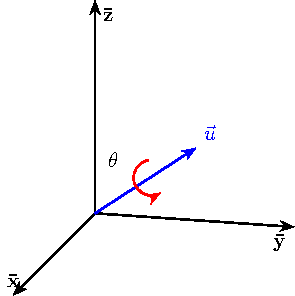
\includegraphics[width=0.3\linewidth]{figures/Quaternion.pdf}
    \caption{Quaternion Rotation}
    \label{fig:3.2}
\end{figure}

\noindent The DCM as a function of Quaternion set is expressed as,

\begin{equation}
    \mathbf{A}_{\mathcal{O}}^{\mathcal{B}} = 
    \begin{bmatrix}
    q_s^2 + q_x^2 - q_y^2 - q_z^2 & 2(q_x q_y - q_s q_z) & 2(q_x q_z + q_s q_y) \\
    2(q_x q_y + q_s q_z) & q_s^2 - q_x^2 + q_y^2 - q_z^2 & 2(q_y q_z - q_s q_x) \\
    2(q_x q_z - q_s q_y) & 2(q_y q_z + q_s q_x) & q_s^2 - q_x^2 - q_y^2 + q_z^2   
    \end{bmatrix}
\end{equation}

\noindent Using the normalisation constraint, $q_s^2 + q_x^2 + q_y^2 + q_z^2 = 1$, the DCM Simplifies to,

\begin{equation}
    \mathbf{A}_{\mathcal{O}}^{\mathcal{B}} = 
    \begin{bmatrix}
    1 - 2(q_y^2 + q_z^2) & 2(q_x q_y - q_s q_z) & 2(q_x q_z + q_s q_y) \\
    2(q_x q_y + q_s q_z) & 1 - 2(q_x^2 + q_z^2) & 2(q_y q_z - q_s q_x) \\
    2(q_x q_z - q_s q_y) & 2(q_y q_z + q_s q_x) & 1 - 2(q_x^2 + q_y^2)   
    \end{bmatrix}
\end{equation}

\noindent The body-fixed angular rates of the satellite in ORB, $\mathbf{\omega}_{\mathcal{B/O}}$, is expressed as a function of qauternions by,

\begin{equation}
    \mathbf{\omega}_\mathcal{B/O} = 
    \begin{bmatrix}
        \omega_{bx} \\ \omega_{by} \\ \omega_{bz}
    \end{bmatrix}
    = 2
    \begin{bmatrix}
       -q_x & q_s & -q_z & q_y \\
       -q_y & q_z & q_s & -q_x \\
       -q_z & -q_y & q_x & q_s 
    \end{bmatrix}
    \begin{bmatrix}
        \dot{q_s} \\ \dot{q_x} \\ \dot{q_y} \\ \dot{q_z}
    \end{bmatrix}
\end{equation}

\noindent Inversly the quaternion rates as a function of the body rates are,

\begin{equation}
    \begin{bmatrix}
        \dot{q_s} \\ \dot{q_x} \\ \dot{q_y} \\ \dot{q_z}
    \end{bmatrix}
    =
    \frac{1}{2}
    \begin{bmatrix}
        0 & -\omega_{bx} & -\omega_{by} & -\omega_{bz}\\
        \omega_{bx} & 0 & \omega_{bz} & -\omega_{by}\\
        \omega_{by} & -\omega_{bz} & 0 & \omega_{bx}\\
        \omega_{bz} & \omega_{by} & -\omega_{bx} & 0 
    \end{bmatrix}
    \begin{bmatrix}
        q_s \\ q_x \\ q_y \\ q_z
    \end{bmatrix}
\end{equation}

\noindent Throughout this thesis, quaternions serve as the primary attitude representation method. Quaternions eliminate rotational sequence 
ambiguities and define rotations about a clearly specified axis. The trigonometric components of the rotation matrix are inherently embedded 
within the quaternion-based DCM formulation. Consequently, attitude transformations require only a single matrix operation using quaternions, whereas 
Euler angle representations necessitate three separate operations.

%=====================================================================================================================================================================================

\mysubsection{Dynamics}{Dynamics}
\label{sec:dynamics}

\mysubsubsection{Translational Dynamics}{Translational Dynamics}

For the translational dynamics, Newton's second law governs the linear motion of the satellite with mass $m$. The discrete-time position and velocity propagation equations are:

\begin{align}
\mathbf{r}_t &= \mathbf{r}_{t-1} + \mathbf{v}_t\Delta t + \frac{1}{2m}\mathbf{F}(t)\Delta t^2 \\
\mathbf{v}_t &= \mathbf{v}_{t-1} + \frac{1}{m}\mathbf{F}(t)\Delta t
\end{align}

\noindent where $\mathbf{F}$ denotes the resultant external force applied to the satellite. 
Within the orbital regime examined in this study, external disturbances are considered insignificant relative to 
gravitational effects. Additionally, given the potential unavailability of precise mass characteristics, the translational dynamics 
may be adequately represented through kinematic approximations wherein the instantaneous velocity is predominantly governed by the preceding velocity state.
\vspace{0.5cm}

\noindent In orbital mechanics, the gravitational force $\mathbf{F}$ acting on a spacecraft is 
proportional to its position vector $\mathbf{r}$ relative to the center of mass. This force is described by the following equation, 
where $\boldsymbol{\mu}$ denotes Earth’s gravitational parameter:


\begin{align}
    \ddot{\mathbf{r}} = \mathbf{F}\mathbf{u}_r \\
    \ddot{\mathbf{r}} = \frac{-\mu}{||\mathbf{r}||^3}\mathbf{u}_r
\end{align}


\noindent The acceleration of a spacecraft in orbit is influenced by several factors, including the primary gravitational 
force $\mathbf{F}_G$, the $J_2$ perturbation $\mathbf{F}_{J2}$, atmospheric drag $\mathbf{F}_{\text{drag}}$, solar radiation 
pressure $\mathbf{F}_{\text{sol}}$, and other miscellaneous perturbations $\mathbf{F}_{\text{misc}}$.
\vspace{0.5cm}

\noindent The total force acting on the satellite can therefore be expressed as:
\begin{align}
    \mathbf{F}_{total} = \mathbf{F}_{G} + \mathbf{F}_{J2} + \mathbf{F}_{drag} + \mathbf{F}_{sol} + \mathbf{F}_{misc}
\end{align}

\noindent However, since we are only modeling Low Earth Orbits (LEO) over a short time period, only the primary gravitational force $\mathbf{F}_G$ and the $J_2$ 
perturbation $\mathbf{F}_{J2}$ are considered.

\noindent The $J_2$ perturbation, which accounts for the Earth's oblateness, is modeled in the Earth-Centered Inertial (ECI) frame using the following equation:

\begin{equation}
\mathbf{a}_{J2} = \frac{3}{2}*J_2*\frac{\mu R_E}{||\mathbf{r}||^5}
\begin{bmatrix}r_x(1-5\frac{z^2}{r^2}) \\
 r_y(1-5\frac{z^2}{r^2})\\
 r_z(3-5\frac{z^2}{r^2}) \end{bmatrix}
\end{equation}

\noindent In this equation, $\mu$ represents Earth's gravitational parameter, $R_E$ is the 
mean radius of the Earth, $J_2$ is the second zonal harmonic coefficient accounting for the Earth's 
oblateness, and $\mathbf{r}$ denotes the satellite's position vector expressed in the Earth-Centered Inertial (ECI) frame.

\mysubsubsection{Rotational Dynamics}{Rotational Dynamics}

The rotational dynamics of a rigid satellite are governed by the Newton-Euler equations, which apply to all rigid inertial bodies.
 The angular momentum $\mathbf{H}$ of the satellite is expressed as:

\begin{equation}
\dot{\mathbf{H}} = \frac{d\mathbf{H}}{dt} = \mathbf{I}\dot{\boldsymbol{\omega}}
\end{equation}

\noindent where $\mathbf{H}$ is the angular momentum vector, $\boldsymbol{\omega}$ is the angular velocity vector expressed in the body 
frame, and $\mathbf{I}$ is the diagonalized moment of inertia tensor about the satellite's principal axes.
\vspace{0.5cm}

\noindent In the absence of external torques, the rotational motion about the satellite's center of mass can be described by Euler's equations:

\begin{align}
I_{xx} \dot{\omega}_x &= \omega_y \omega_z (I_{yy} - I_{zz}) \\
I_{yy} \dot{\omega}_y &= \omega_x \omega_z (I_{zz} - I_{xx}) \\
I_{zz} \dot{\omega}_z &= \omega_x \omega_y (I_{xx} - I_{yy})
\end{align}

\noindent where $I_{xx}$, $I_{yy}$, and $I_{zz}$ are the principal moments of inertia, which are constant and determined by the satellite's mass distribution and geometry.
\vspace{0.5cm}

\noindent The stability of the satellite's rotational motion is influenced by its moment of inertia. According to Marsden and Ratiu, rotation about the 
major or minor principal axis is stable, while rotation about the intermediate axis is inherently unstable. Under constant energy conditions, any 
initial rotation around the intermediate axis will tend to redistribute energy toward the major and minor axes due to nutation effects.
\vspace{0.5cm}

\noindent To propagate the satellite's attitude over time, the quaternion derivative must be computed. The quaternion $\mathbf{q}_{B/I}$, which represents the 
rotation from the inertial frame to the body frame, evolves according to:

\begin{equation}
\dot{\mathbf{q}}_{B/I} = \frac{1}{2}(\mathbf{q}_{B/I} \otimes \boldsymbol{\omega})
\end{equation}

\noindent where $\boldsymbol{\omega} = [\omega_x, \omega_y, \omega_z]^T$ is the angular velocity vector in the body frame, and $\otimes$ denotes 
quaternion multiplication. Expanding this yields:

\begin{equation}
\dot{\mathbf{q}}_{B/I} = \frac{1}{2}
\begin{bmatrix}
q_{B/I,0} \omega_x - q_{B/I,3} \omega_y + q_{B/I,2} \omega_z \\
q_{B/I,3} \omega_x + q_{B/I,0} \omega_y - q_{B/I,1} \omega_z \\
-q_{B/I,2} \omega_x + q_{B/I,1} \omega_y + q_{B/I,0} \omega_z \\
-q_{B/I,1} \omega_x - q_{B/I,2} \omega_y - q_{B/I,3} \omega_z
\end{bmatrix}
\end{equation}

\noindent where $q_{B/I,0}$ is the scalar part and $q_{B/I,1}, q_{B/I,2}, q_{B/I,3}$ are the vector components of the quaternion.
\vspace{0.5cm}

\noindent Quaternion propagation is performed using a simple Euler integration scheme. First, the quaternion is advanced in time as:

\begin{equation}
\bar{\mathbf{q}}_{B/I}(t + \Delta t) = \mathbf{q}_{B/I}(t) + \dot{\mathbf{q}}_{B/I} \Delta t
\end{equation}

\noindent where $\bar{\mathbf{q}}_{B/I}$ is the unnormalized quaternion. To maintain a valid attitude representation, the quaternion must be renormalized:

\begin{equation}
\mathbf{q}_{B/I}(t + \Delta t) = \frac{\bar{\mathbf{q}}_{B/I}(t + \Delta t)}{||\bar{\mathbf{q}}_{B/I}(t + \Delta t)||}
\end{equation}

\noindent This normalization step ensures that the quaternion maintains unit magnitude throughout integration.

\mysection{Refrence Frame Transformations}{Refrence Frame Transformations}

In this project, several different reference frames will be encountered. To accurately construct the measurement model, it is 
essential to understand each of these reference frames and the transformations between them.

\mysubsection{Transformation Matrix}{Transformation Matrix}

Transformations between different reference frames are a fundamental part of spacecraft modeling and sensor simulation. These 
transformations are typically expressed using homogeneous transformation matrices, which combine both rotation and translation components 
into a single $4 \times 4$ matrix.

\mysubsubsection{Rotation Matrix}{Rotation Matrix}

In many practical scenarios, such as pure attitude transformations or body-to-inertial frame conversions, only rotational 
alignment is needed. In such cases, only the DCM $\mathbf{A}$ is used like discussed in previous chapters, and the transformation is defined as:

\begin{equation}
    \mathbf{v}_\mathcal{O} = \mathbf{A}_\mathcal{I}^\mathcal{O} \cdot \mathbf{v}_\mathcal{I}
\end{equation}

\noindent Note that:

\begin{equation}
    \mathbf{A}_\mathcal{I}^\mathcal{O} = \left( \mathbf{A}_\mathcal{O}^\mathcal{I} \right)^\top
\end{equation}

\noindent and that the reverse rotation can be applied.

\begin{equation}
    \mathbf{v}_\mathcal{I} = \left(\mathbf{A}_\mathcal{I}^\mathcal{O}\right)^T \cdot \mathbf{v}_\mathcal{O}
\end{equation}

\noindent This relationship arises because direction cosine matrices are orthogonal.

\mysubsubsection{Translation}{Translation}

In many of the reference frames the translation of the origin is required, To translate from one refrence frame the the other

\begin{equation}
    \mathbf{v}_\mathcal{B/I} = \mathbf{v}_\mathcal{B} - \mathbf{r}_\mathcal{I}
\end{equation}

\noindent Where $\mathbf{v}_\mathcal{B/I}$ is the vector in $\mathcal{B}$ relative to $\mathcal{I}$ and $\mathbf{v}_\mathcal{B}$ is the vector in 
the body frame and $\mathbf{r}_\mathcal{I}$ is the position of the Body frame origin in the inertial reference frame.

\mysubsubsection{Homogeneous Transformation Matrix}{Homogeneous Transformation Matrix}

\noindent A homogeneous transformation matrix from $\mathcal{I}$ to $\mathcal{O}$ is defined as:

\begin{equation}
    \mathbf{T}_\mathcal{I}^\mathcal{O} =
    \begin{bmatrix}
        \mathbf{A}_\mathcal{I}^\mathcal{O} & -\mathbf{A}_\mathcal{I}^\mathcal{O} \cdot \mathbf{r}_\mathcal{I} \\
        \mathbf{0}_{1 \times 3} & 1
    \end{bmatrix}
\end{equation}

\noindent Here, $\mathbf{A}_\mathcal{I}^\mathcal{O}$ is a $3 \times 3$ direction cosine matrix (DCM) that describes the orientation of frame $\mathcal{O}$ 
relative to frame $\mathcal{I}$, and $\mathbf{r_I}$ is a translation vector from the origin of $\mathcal{I}$ to the origin of $\mathcal{O}$, expressed 
in frame $\mathcal{I}$.

\noindent This formulation ensures that both the direction and magnitude of vectors are preserved during the transformation. However, it is important to note 
that the inverse transformation is \textbf{not} obtained from getting the transpose.

\begin{equation}
    \mathbf{T}_\mathcal{I}^\mathcal{O} \ne \left(\mathbf{T}_\mathcal{O}^\mathcal{I}\right)^T
\end{equation}

\mysubsection{Lattitude, longitude and altitude}{Lattitude, longitude and altitude}

The lattitude, longitude and altitude of a feature or the position of the satellite is donated with the $\mathcal{L}$. The lattitude of a feature is the position of how high or low it above the
equator, having a range of $-90^{\circ}$ to $90^{\circ}$. The longitude is based of the greenwich maridian, a longitude line that pases through the north- and south pole, it has a
range of $-180^{\circ}$ to $180^{\circ}$. The altitude is measured form the the "WGS84" elliptical globe.

\begin{equation}
    \mathbf{r}_\mathcal{L} = \begin{bmatrix}
    \lambda \\
    \phi \\
    h    
    \end{bmatrix} 
\end{equation}

\mysubsection{Earth Cenetered Earth Fixed}{Earth Cenetered Earth Fixed}

The Earth Centered Earth Fixed also known as Earth Centered Rotating (ECR) refrence frame is represented by the $\mathcal{R}$ and is very simular to the $\mathcal{L}$ reference
 frame with the z-axis alligned with the northpole and the x-axis points at the crossing of the Prime Maridian an the Equator, where the y-axis completes the right hand rule. The x,y and z-axis is defined in kilometers.
To covert from $\mathcal{L}$ to $\mathcal{R}$ is to use a "WGS84" transfomr. Where WGS84 stands for World Geodetic System 1984, which is the standard coordinate system used for
Global Positioning System (GPS). The WGS84 transformation uses a reference ellipsoid that uses a semi-major axis of 6,378 km and a flatting of 1/298.2 .

\begin{equation}
        \mathbf{T}_{\mathcal{L}}^{\mathcal{F}} = f(\text{WGS84})
\end{equation}

\begin{figure}[H]
    \centering
    \begin{subfigure}[t]{0.45\textwidth}
        \centering
        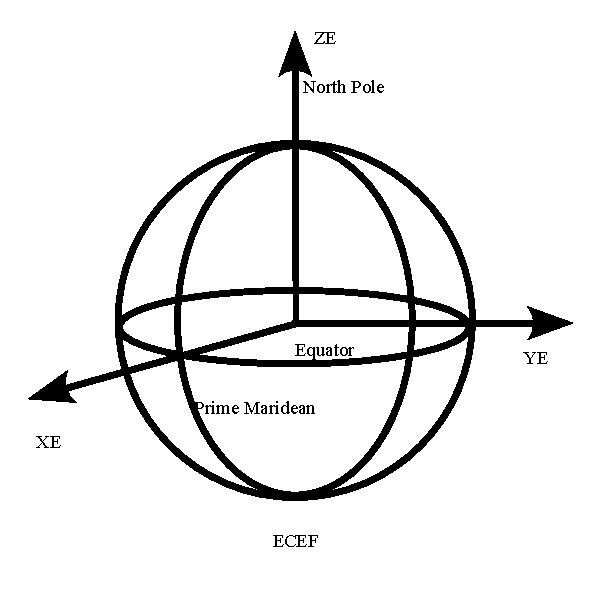
\includegraphics[width=\textwidth]{figures/modelling/ECEF.pdf}
        \caption{The Earth-Centered, Earth-Fixed (ECEF) reference frame.}
        \label{fig:ecef}
    \end{subfigure}
    \hfill
    \begin{subfigure}[t]{0.45\textwidth}
        \centering
        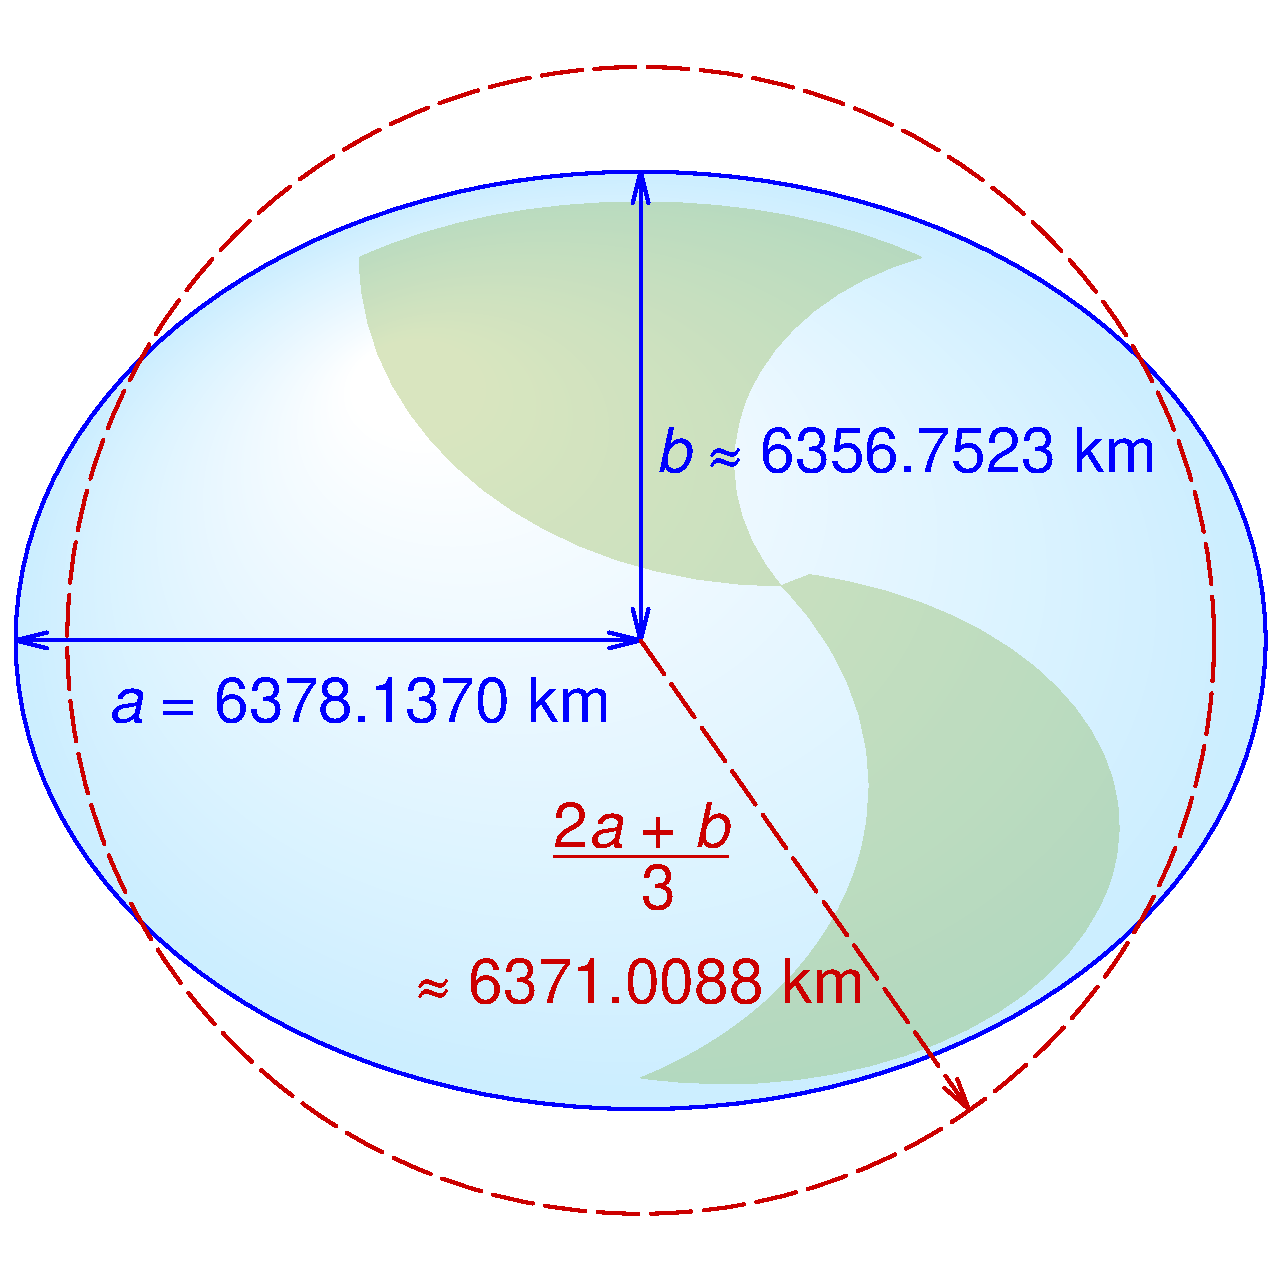
\includegraphics[width=\textwidth]{figures/modelling/WGS84_mean_Earth_radius.pdf}
        \caption{WGS84 model showing the mean Earth radius.}
        \label{fig:wgs84}
    \end{subfigure}
    \caption{Geodetic reference frames and models used in Earth observation.}
    \label{fig:geodetic-frames}
\end{figure}


\begin{figure}[H]
    \centering
    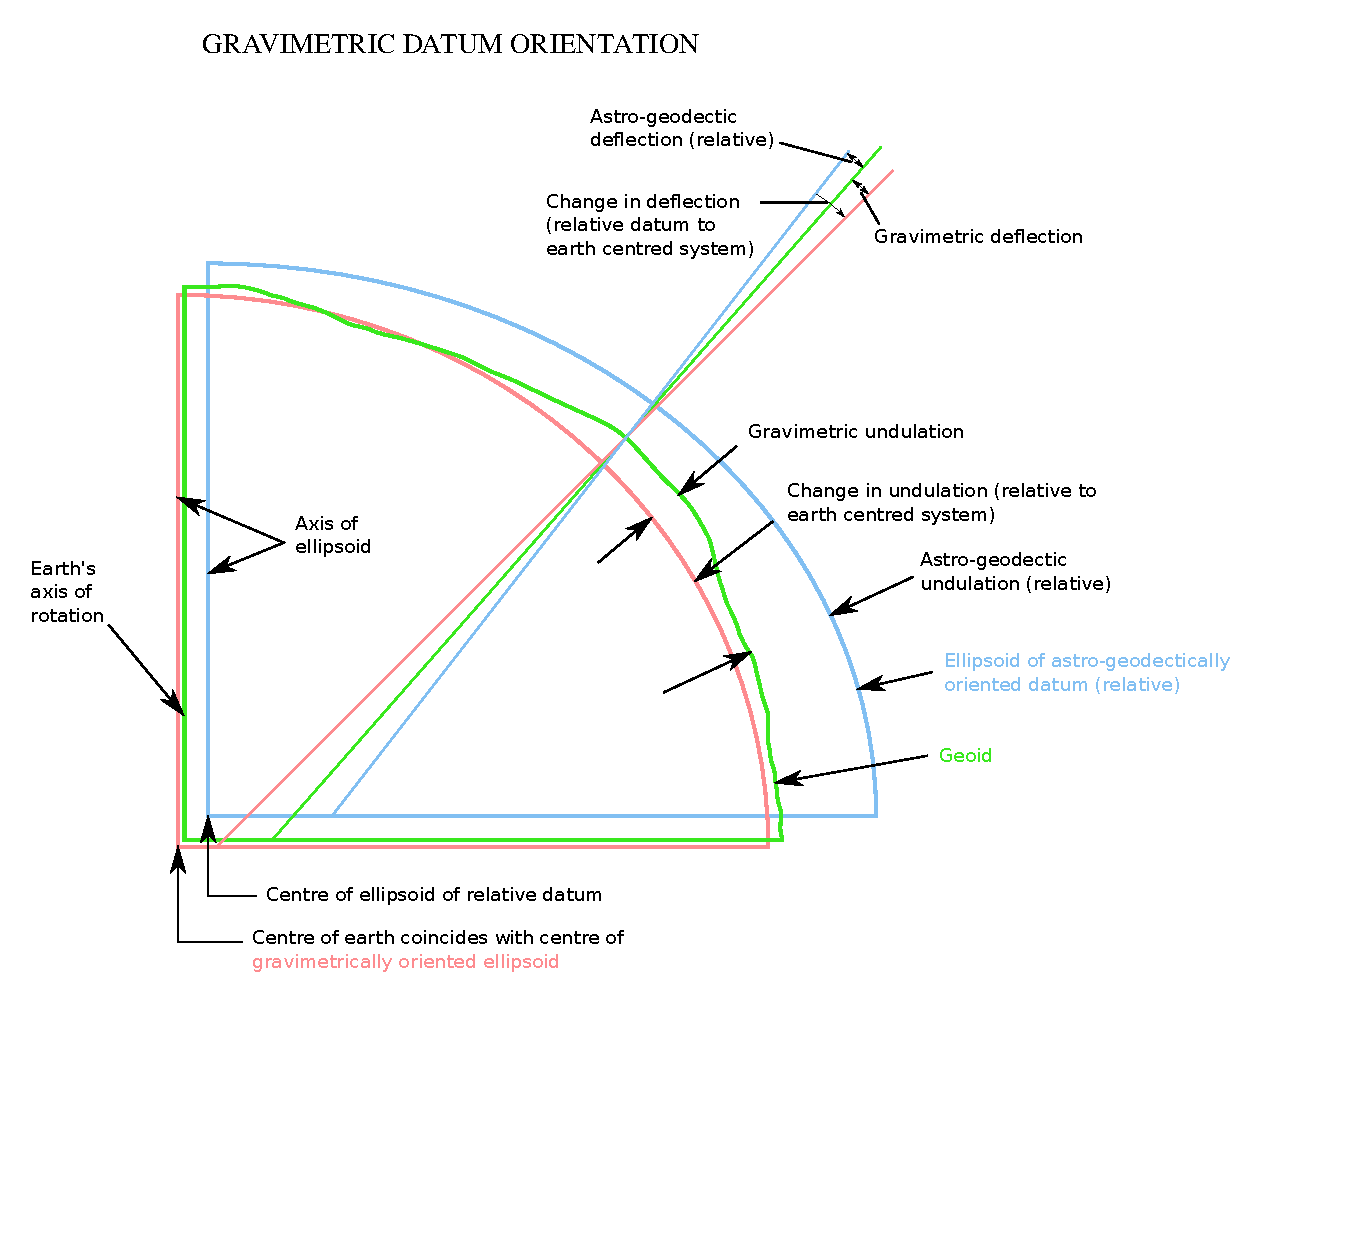
\includegraphics[width=\textwidth]{figures/modelling/GRAVIMETRIC_DATUM_ORIENTATION}
    \caption{The Earth Cetred Earth Fixed reference frame}
    \label{fig:3.4}
\end{figure}




\mysubsection{Earth Centered Inertial}{Earth Ceneterd Inertial}

The Earth Centered Inertial refrence fream (ECI) refrenced by $\mathcal{I}$ shares a refrence frame axis with the ECEF, but is rotated about the z-axis. The Earth
Centered refrence frame is defined as the x-axis pointing in the direction where the equatorial plane and the ecliptic plane cross, also known as the Vernal equanox, the
z-axis is degined as the north pole and the Y axis completes the right hadn rule. This rotation is governed by the rotation speed of the earth $\omega_e$ which 
is $7.2921\times10^{-5}$ rad/s and time $t$. To transform from the ECEF reference frame to the ECI reference frame one shouldrotate the Earth clockwise e.i. 

\begin{equation}
    \mathbf{A}_{\mathcal{F}}^{\mathcal{I}} = R(\omega_e t) = 
    \begin{bmatrix}
        \cos(-\omega_e t) & -\sin(-\omega_e t) & 0\\
        \sin(-\omega_e t) & \cos(-\omega_e t) & 0\\
        0 & 0 & 1
    \end{bmatrix}
\end{equation}

\begin{figure}[H]
    \centering
    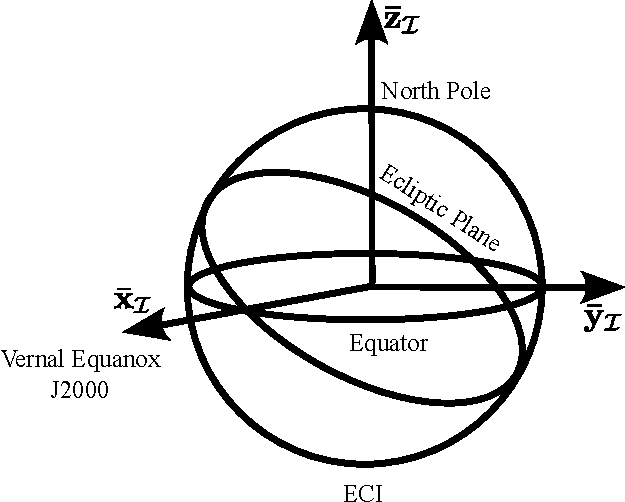
\includegraphics[width=0.4\textwidth]{figures/modelling/ECI.pdf}
    \caption{Earth Centered Earth Inertial Reference Frame}
    \label{fig:3.5}
\end{figure}

\mysubsection{Orbital reference frame}{Orbital reference frame}

The orbital reference frame used is the Local Vertical Local Horizon (LVLH) denoted by $\mathcal{O}$.The LVLH frame is a rotating, orbit-attached corrdinate
system commonly used in spacecraft dynamics. It moves with the satellite and is defined relative to its orbit around Earth. The z-axis is the local vertical and is also called the Nadir direction, 
it points to the barycenter of the system, in this case the center of the Earth. The y-axis is called the cross track t points 
out of the orbital plane, typically the anti-angular momentum vector direction (anti-normal to the orbit plane). The x-axis is the "Local Horizon" also called
"along track" pointing forward it is tangent to the orbit and completes the right hand rule.
\vspace{0.5cm}

\noindent If $\mathbf{r}$ is the position vector of the satellite and $\mathbf{v}$ is the velocity vector of the satellite.
The equation for the reference frame is:

\begin{align}
    \bar{z}_{\mathcal{O}} &= -\frac{\mathbf{r}}{||\mathbf{r}||} \\
    \bar{y}_{\mathcal{O}} &= \frac{\mathbf{r}\times\mathbf{v}}{||\mathbf{r}\times\mathbf{v}||}\\
    \bar{x}_{\mathcal{O}} &= \bar{y}_{\mathcal{O}}\times\bar{z}_{\mathcal{O}}
\end{align}

\noindent For this reference frame there should also be a refrence frame translation introduced. Which is done by substracing $\mathbf{r}$ from the vector

\begin{equation}
    \mathbf{f}_{\mathcal{O}} = \mathbf{A}_{\mathcal{I}}^{\mathcal{O}}\times(\mathbf{f}_{\mathcal{I}} - \mathbf{r}_{\mathcal{I}})
\end{equation}

\begin{figure}[H]
    \centering
    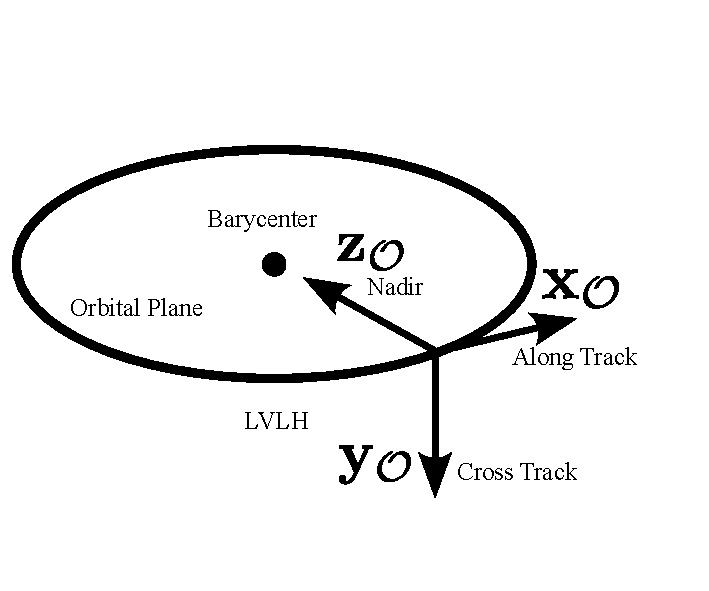
\includegraphics[width=0.4\textwidth]{figures/modelling/LVLH.pdf}
    \caption{The Orbital Reference frame (also known as the LVLH)}
    \label{fig:3.6}
\end{figure}

\subsection{Body Referenece frame}

The body reference frame denoted by $\mathcal{B}$ is the reference frame of the satellite body itself, with the center point referenced as the center of mass of the satellite body.
with the z-axis defined as the yaw, x-axis defined as the roll and the y-axis defined as the pitch of the satellite. With the body frame z-axis and the orbital reference frame 
as alligned at initialisiation


\begin{figure}[H]
    \centering
    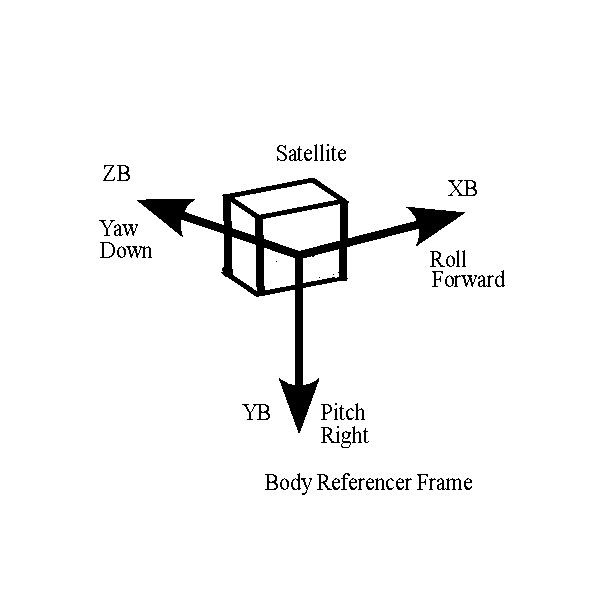
\includegraphics[width=0.5\textwidth]{figures/modelling/BRF.pdf}
    \caption{}
    \label{fig:BRF}
\end{figure}



\mysection{Sensor Modelling}{Sensor Modelling}

\mysubsection{GPS Measurement Model}{GPS Measurement Model}

In the simulation, GPS measurements are generated using the same underlying dynamics as the truth model, which is based 
on the two-body problem. This ensures consistency between the true satellite motion and the measurement framework. However, to emulate realistic 
sensor behavior, the GPS measurements are corrupted by both noise and drift.
\vspace{0.5cm}

\noindent One of the GPS sensor outputs is called \$GPGGA which contains the tim, lattitude, longitude and altitude data. To model this measurement 
the simualted measurement $\mathbf{x}_{\text{true},\text{pos}}$ needs to be converted to a the $\mathcal{L}$ representation

\begin{equation}
    \mathbf{x}_{\text{true},\text{pos},\mathcal{L}} = f(\text{WGS84},\mathbf{A}_\mathcal{I}^\mathcal{R},\mathbf{x}_{\text{true},\text{pos},\mathcal{I}})
\end{equation}

\noindent The GPS measurement model is expressed as:
\begin{equation}
    \mathbf{z}_{GPS}(t) = \mathbf{x}_{\text{true}}(t) + \boldsymbol{\eta}_{GPS}(t) + \mathbf{d}_{GPS}(t),
\end{equation}

\noindent Let $\mathbf{z}_{GPS}(t)$ denote the observed GPS measurement at time $t$, which is modeled as the sum of the true system state $\mathbf{x}_{\text{true}}(t)$, 
as propagated by the two-body equations of motion, additive zero-mean Gaussian measurement noise $\boldsymbol{\eta}_{GPS}(t)$, and a GPS drift component $\mathbf{d}_{GPS}(t)$.
\vspace{0.5cm}

\noindent The drift component models the slow, unbounded accumulation of error that is characteristic of certain classes of low-cost GPS receivers. 
It is implemented as a random walk process:
\begin{equation}
    \mathbf{d}_{GPS}(t) = \mathbf{d}_{GPS}(t - \Delta t) + \mathbf{q}_{GPS}(t),
\end{equation}


\noindent Here, $\mathbf{d}_{GPS}(t - \Delta t)$ represents the GPS drift at the previous timestep, and $\mathbf{q}_{GPS}(t)$ is a zero-mean stochastic increment that models the drift rate. This increment is typically drawn from a Gaussian distribution, given by
\begin{equation}
    \mathbf{q}_{GPS}(t) \sim \mathcal{N}(0, \sigma_d^2 \mathbf{I}).
\end{equation}


\noindent This formulation captures both short-term measurement variability through $\boldsymbol{\eta}_{GPS}(t)$ and long-term bias trends 
via $\mathbf{d}_{GPS}(t)$, allowing for more realistic testing and evaluation of estimation algorithms under degraded or imperfect sensing conditions.
\begin{figure}[H]
    \centering
    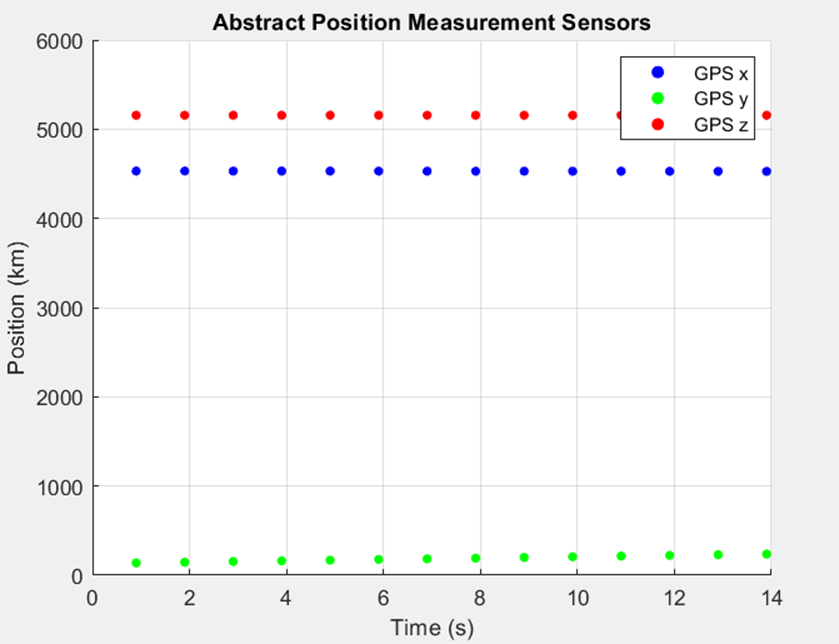
\includegraphics[width=0.4\textwidth]{figures/modelling/GPSMeasurement.png}
    \caption{}
    \label{fig:GPS}
\end{figure}



\textcolor{blue}{Insert Image of Modelled GPS Results}

\mysubsection{Gyroscope Measuement Model}{Gyroscope Measurement Model}

The gyroscope provides a measurement of the angular velocity of the body frame relative to the inertial frame, expressed in the body frame. This quantity is denoted as $\boldsymbol{\omega}^B_{B/I}$, and forms a critical part of attitude determination and estimation systems.

To simulate a realistic sensor, the gyroscope measurement is corrupted by both random noise and a time-varying bias, or drift. The measurement model is given by:

\begin{equation}
    \mathbf{z}_{\text{Gyro}}(t) = \boldsymbol{\omega}^B_{B/I}(t) + \boldsymbol{\eta}_{\text{Gyro}}(t) + \mathbf{d}_{\text{Gyro}}(t),
\end{equation}

where:
\begin{itemize}
    \item $\mathbf{z}_{\text{Gyro}}(t)$ is the observed gyroscope measurement at time $t$,
    \item $\boldsymbol{\omega}^B_{B/I}(t)$ is the true angular velocity of the body frame relative to the inertial frame,
    \item $\boldsymbol{\eta}_{\text{Gyro}}(t)$ is zero-mean Gaussian noise representing short-term measurement error, and
    \item $\mathbf{d}_{\text{Gyro}}(t)$ is the gyroscope drift, modeled as a time-varying bias.
\end{itemize}

The drift is modeled as a random walk process, capturing slow variations in the sensor bias over time:

\begin{equation}
    \mathbf{d}_{\text{Gyro}}(t) = \mathbf{d}_{\text{Gyro}}(t - \Delta t) + \mathbf{q}_{\text{Gyro}}(t),
\end{equation}

with the stochastic increment defined as:

\begin{equation}
    \mathbf{q}_{\text{Gyro}}(t) \sim \mathcal{N}(0, \sigma_g^2 \mathbf{I}),
\end{equation}

where $\sigma_g^2$ represents the drift rate variance of the gyroscope.

This model allows for the representation of both high-frequency noise and long-term integration drift, which are commonly observed in practical inertial measurement units (IMUs). Incorporating this model into the estimation framework enables more robust and accurate state reconstruction in the presence of sensor imperfections.




\mysubsection{Star Tracker}{Star Tracker}


The Star Tracker (ST) is a high-accuracy attitude sensor that provides an absolute measurement of the spacecraft's orientation, typically in quaternion form. Unlike relative sensors such as gyroscopes, the Star Tracker outputs an independent estimate of the spacecraft’s attitude by capturing star field images and comparing them to a catalog.

In this simulation, the Star Tracker measurement is generated by perturbing the true attitude quaternion with a small random rotation. This models the sensor's measurement noise, which is assumed to follow a zero-mean Gaussian distribution.

\paragraph{Noise Quaternion Generation}

To simulate this noise, a small random rotation axis is sampled from a standard normal distribution and normalized. A noise quaternion $\mathbf{q}_{\text{noise}}$ is then constructed from this axis and a given angular noise magnitude $\theta$ (specified in degrees):

\begin{equation}
    \mathbf{q}_{\text{noise}} = 
    \begin{bmatrix}
        \cos\left(\frac{\theta}{2}\right) \\
        \hat{\mathbf{u}} \sin\left(\frac{\theta}{2}\right)
    \end{bmatrix}
\end{equation}

where $\hat{\mathbf{u}}$ is a unit vector sampled from $\mathcal{N}{(0,1)}^3$ and $\theta = \deg2rad(ST_{\text{noise}})$.

\paragraph{Measurement Model}

The measured Star Tracker quaternion is computed by applying the noise quaternion to the true attitude quaternion using the Hamilton product:

\begin{equation}
    \mathbf{z}_{ST} = \mathbf{q}_{\text{noise}} \otimes \mathbf{q}_{\text{true}}
\end{equation}

This represents a small perturbation of the true attitude, emulating realistic sensor output.

This model captures the key behavior of a real Star Tracker by applying small rotational noise to the true spacecraft attitude. 
It is suitable for use in truth-model simulations and Kalman filter evaluations, providing high-fidelity yet controllable measurement uncertainty.


\textcolor{blue}{Add Some Results}


\mysubsection{Coarse Sun Senser}{Coarse Sun Sensor}
\label{sec:css}

The Coarse Sun Sensor (CSS) is a fundamental attitude sensing instrument in nanosatellite systems, providing an estimate of the Sun direction relative to the satellites body frame. This subsection outlines the modeling approach for simulating CSS measurements, including the transformation of reference frames, sensor configuration, noise characteristics, and estimation logic.

\paragraph{Sun Vector in Inertial Frame}

The Sun vector is modeled in the Earth-Centered Inertial (ECI) frame as a fixed unit vector pointing in the $+X$ direction:

\begin{equation}
    \mathbf{S}_\mathcal{I} = \begin{bmatrix} 1 & 0 & 0 \end{bmatrix}^\top
\end{equation}

This simplified model assumes that the Sun direction does not vary during the simulation.

\paragraph{Transformation to Body Frame}

To simulate the Sun vector in the satellite’s body frame, the inertial vector is rotated using the satellite's true attitude quaternion. The corresponding direction cosine matrix (DCM) is derived as:

\begin{equation}
     \mathbf{S}_\mathcal{B} = R_I^B \cdot \mathbf{S}_\mathcal{I}
\end{equation}

where $R_I^B$ is the DCM from the inertial to body frame.

\paragraph{Sensor Layout and Response}

The CubeSat is equipped with six coarse sun sensors, one on each face, aligned along the $\pm X$, $\pm Y$, and $\pm Z$ body axes (see Figure~\ref{fig:CSS}). Each sensor has a cosine response:

\begin{equation}
     z_i = \max\left(0, \hat{\mathbf{n}}_i^\top \mathbf{S}_\mathcal{B} \right), \quad i = 1, \dots, 6
\end{equation}

where $\hat{\mathbf{n}}_i$ is the normal vector of the $i$-th sensor surface.

\begin{figure}[H]
    \centering
    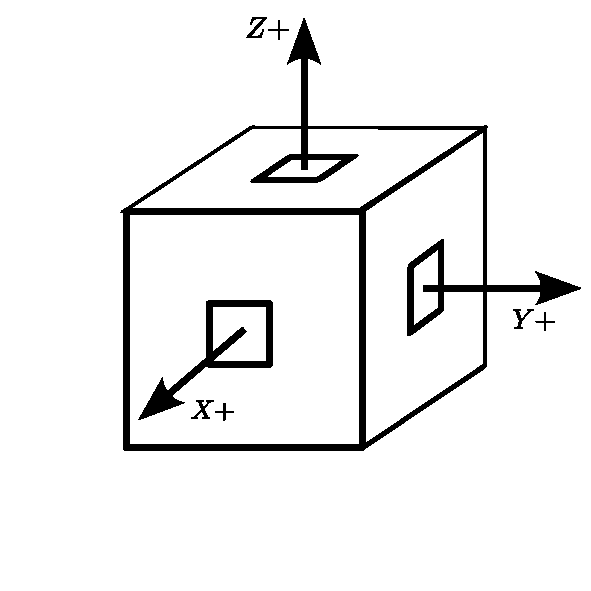
\includegraphics[width=0.4\textwidth]{figures/modelling/CSS.pdf}
    \caption{Orientation of the six coarse sun sensors on the CubeSat}
    \label{fig:CSS}
\end{figure}

\paragraph{Measurement Noise}

Each CSS reading is perturbed with zero-mean Gaussian noise. The noise standard deviation $\sigma$ is specified in degrees and converted to radians:

\begin{equation}
    \mathbf{z}_{\text{CSS}} = \max\left( 0, \mathbf{z}_{\text{CSS}} + \mathcal{N}(0, \sigma^2) \right), \quad \sigma = \deg2rad(\text{CSS}_{\text{noise}})
\end{equation}

Negative readings are clamped to zero since physical sensors cannot detect negative intensity.

\paragraph{Sun Vector Estimation}

The estimated Sun vector in the body frame is reconstructed using a weighted sum of the face normals:

\begin{equation}
    \hat{\mathbf{S}}_\mathcal{B} = \sum_{i=1}^{6} z_i \cdot \hat{\mathbf{n}}_i
\end{equation}

The result is normalized to produce a unit vector:

\begin{equation}
    \hat{\mathbf{S}}_\mathcal{B} = \frac{\hat{\mathbf{S}}_\mathcal{B}}{|\hat{\mathbf{S}}_\mathcal{B}|}
\end{equation}


\textcolor{blue}{Add some results}

\mysubsection{Magnetometer}{Magnetometer}

The magnetometer measurement is modeled as a unit vector pointing along the direction of the Earth's magnetic field as observed from the satellite body frame. To approximate this field, a simplified model is used in which the magnetic field points toward the geographic North Pole and is tangential to the Earth's surface at the satellit's location, with an optional dip angle to simulate inclination.

\textbf{Step 1: Earth-Fixed Transformation}

To determine the orientation of the magnetic field relative to the Earth-fixed frame, the satellite position vector $\mathbf{r}_{\mathcal{I}}$ in the inertial (ECI) frame is first transformed to the Earth-fixed (ECEF) frame using a rotation matrix that accounts for Earth's rotation angle at time $t$:

\begin{equation}
    \mathbf{r}_{\mathcal{R}} = R_{\mathcal{I}}^{\mathcal{R}}(t) \cdot \mathbf{r}_{\mathcal{I}}
\end{equation}

where $R_{\mathcal{I}}^{\mathcal{R}}(t)$ is a time-dependent rotation matrix based on the Earth rotation rate $\omega_e$.

\textbf{Step 2: Direction to Magnetic North}

The geographic North Pole is approximated by a fixed point on the Z-axis of the Earth-fixed frame:

\begin{equation}
    \mathbf{p}_{NP,\mathcal{R}} = \begin{bmatrix} 0 \\ 0 \\ R_E \end{bmatrix}
\end{equation}

The direction vector from the satellite to the North Pole is then computed as:

\begin{equation}
    \mathbf{d}_{NP} = \mathbf{p}_{NP,\mathcal{R}} - \mathbf{r}_{\mathcal{R}}
\end{equation}

\textbf{Step 3: Tangential Magnetic Field Model}

The local radial unit vector from the Earth's center is:

\begin{equation}
    \mathbf{u}_{r,\mathcal{R}} = \frac{\mathbf{r}_{\mathcal{R}}}{|\mathbf{r}_{\mathcal{R}}|}
\end{equation}

To simulate a magnetic field that is tangential to Earth's surface, the component of $\mathbf{d}_{NP}$ in the radial direction is removed:

\begin{equation}
    \mathbf{z}_{\text{Mag},\mathcal{R}} = \mathbf{d}_{NP} - (\mathbf{d}_{NP} \cdot \mathbf{u}_{r,\mathcal{R}})\mathbf{u}_{r,\mathcal{R}}
\end{equation}

This tangential field vector is then normalized:

\begin{equation}
    \mathbf{z}_{\text{Mag},\mathcal{R}} = \frac{\mathbf{z}_{\text{Mag},\mathcal{R}}}{|\mathbf{z}_{\text{Mag},\mathcal{R}}|}
\end{equation}

\begin{figure}[H]
    \centering
    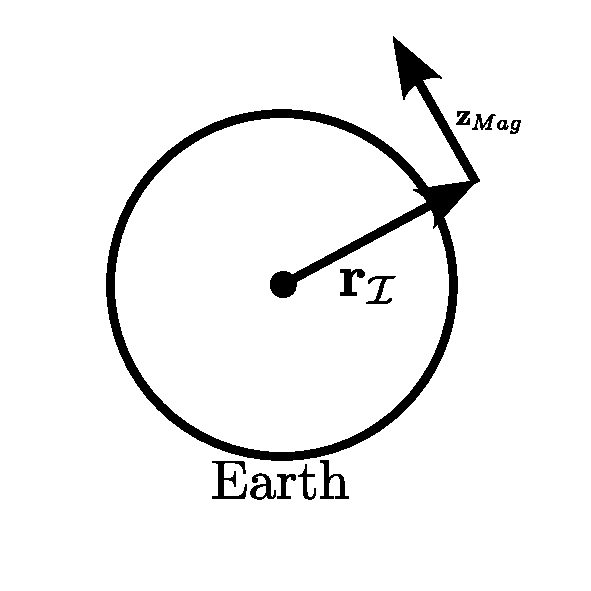
\includegraphics[width=0.4\textwidth]{figures/modelling/Magnetometer.pdf}
    \caption{}
    \label{fig:CSS}
\end{figure}

\textbf{Step 4: Dip Angle Adjustment}

To simulate magnetic inclination, a rotation about the local East direction is applied to tilt the magnetic field by a dip angle $\delta$, which is measured downward from the local horizontal plane:

\begin{equation}
    \mathbf{z}_{\text{Mag},\mathcal{R}}^{\text{incl}} = \cos(\delta)\,\mathbf{z}_{\text{Mag},\mathcal{R}} + \sin(\delta)\,(\mathbf{e}_{\text{East}} \times \mathbf{z}_{\text{Mag},\mathcal{R}})
\end{equation}

Here, $\mathbf{e}_{\text{East}}$ is the local east direction, obtained via:

\begin{equation}
    \mathbf{e}_{\text{East}} = \frac{\mathbf{u}_{r,\mathcal{R}} \times \mathbf{z}_{\text{Mag},\mathcal{R}}}{|\mathbf{u}_{r,\mathcal{R}} \times \mathbf{z}_{\text{Mag},\mathcal{R}}|}
\end{equation}


\textbf{Step 5: Reference Frame Transformations}

The inclined magnetic field vector is transformed back to the inertial frame using:

\begin{equation}
    \mathbf{z}_{\text{Mag},\mathcal{I}} = R_{\mathcal{R}}^{\mathcal{I}}(t) \cdot \mathbf{z}_{\text{Mag},\mathcal{R}}^{\text{incl}}
\end{equation}

The final transformation to the spacecraft body frame is performed using the spacecraft attitude quaternion $\mathbf{q}_{\mathcal{B}}^{\mathcal{I}}$, resulting in:

\begin{equation}
    \mathbf{z}_{\text{Mag},\mathcal{B}} = R(\mathbf{q}_{\mathcal{B}}^{\mathcal{I}}) \cdot \mathbf{z}_{\text{Mag},\mathcal{I}}
\end{equation}

where $R(\mathbf{q})$ is the direction cosine matrix corresponding to the quaternion $\mathbf{q}$.

\textbf{Step 6: Measurement Noise}

To simulate realistic sensor output, a small-angle random rotation is applied to the vector $\mathbf{z}_{\text{Mag},\mathcal{B}}$ to represent magnetometer noise. This is modeled by sampling a noise rotation axis and applying a perturbation angle drawn from a Gaussian distribution with a standard deviation $\sigma_{\text{noise}}$ (in radians). The rotation is implemented via a noise quaternion and applied to the magnetic field vector.

\textbf{Step 7: Output}

The final estimated magnetometer vector $\hat{\mathbf{z}}_{\text{Mag},\mathcal{B}}$ is normalized and output for use in state estimation:

\begin{equation}
    \hat{\mathbf{z}}_{\text{Mag},\mathcal{B}} = \frac{\mathbf{z}_{\text{Mag},\mathcal{B}}}{|\mathbf{z}_{\text{Mag},\mathcal{B}}|}
\end{equation}

This provides a realistic simulation of a three-axis magnetometer, with both geographic dependence and sensor-level noise, for use in spacecraft attitude determination or estimation filters.


\mysubsection{TRIAD Attitude Estimation}{TRIAD Attitude Estimation}

The TRIAD (Tri-Axial Attitude Determination) algorithm is a deterministic method used to estimate a spacecraft's attitude from two independent, non-collinear direction measurements expressed in both the body and inertial frames. In this work, the TRIAD method is applied using sun vector measurements from a coarse sun sensor and magnetic field measurements from a three-axis magnetometer.

\textbf{Step 1: Sensor Measurements in Body Frame}

Let $\mathbf{s}_{\mathcal{B}}$ denote the unit vector pointing toward the Sun in the body frame, and $\mathbf{m}_{\mathcal{B}}$ the unit magnetic field vector in the body frame. These vectors are obtained from sensor measurements and normalized:

\begin{equation}
    \mathbf{s}_{\mathcal{B}} = \frac{\mathbf{s}_{\mathcal{B}}}{|\mathbf{s}_{\mathcal{B}}|}, \quad
    \mathbf{m}_{\mathcal{B}} = \frac{\mathbf{m}_{\mathcal{B}}}{|\mathbf{m}_{\mathcal{B}}|}
\end{equation}

\textbf{Step 2: Reference Vectors in Inertial Frame}

The inertial-frame counterparts to the measured vectors are defined as follows:

- The Sun vector in the inertial (ECI) frame is approximated by the unit vector:

\begin{equation}
   \mathbf{s}_{\mathcal{I}} = \begin{bmatrix} 1 \\ 0 \\ 0 \end{bmatrix}
\end{equation}

- The magnetic field vector in the inertial frame, $\mathbf{m}_{\mathcal{I}}$, is computed based on the spacecraft position $\mathbf{r}_{\mathcal{I}}$, a user-defined magnetic dip angle, and Earth’s rotation:

\begin{equation}
   \mathbf{m}_{\mathcal{I}} = \text{MagnetometerModel}(\mathbf{r}_{\mathcal{I}}, t, \omega_e, \delta)
\end{equation}

Both reference vectors are normalized:

\begin{equation}
   \mathbf{s}_{\mathcal{I}} = \frac{\mathbf{s}_{\mathcal{I}}}{|\mathbf{s}_{\mathcal{I}}|}, \quad
   \mathbf{m}_{\mathcal{I}} = \frac{\mathbf{m}_{\mathcal{I}}}{|\mathbf{m}_{\mathcal{I}}|}
\end{equation}

\textbf{Step 3: Constructing Orthogonal Triads}

Two orthonormal vector triads are constructed from the body and reference measurements.

- In the inertial frame:

\begin{align}
    \mathbf{v}_1^{\mathcal{I}} &= \mathbf{s}_{\mathcal{I}} \\
    \mathbf{v}_2^{\mathcal{I}} &= \frac{\mathbf{s}_{\mathcal{I}} \times \mathbf{m}_{\mathcal{I}}}{|\mathbf{s}_{\mathcal{I}} \times \mathbf{m}_{\mathcal{I}}|} \\
    \mathbf{v}_3^{\mathcal{I}} &= \mathbf{v}_1^{\mathcal{I}} \times \mathbf{v}_2^{\mathcal{I}}
\end{align}

- In the body frame:

\begin{align}
    \mathbf{v}_1^{\mathcal{B}} = \mathbf{s}_{\mathcal{B}} \\
    \mathbf{v}_2^{\mathcal{B}} = \frac{\mathbf{s}_{\mathcal{B}} \times \mathbf{m}_{\mathcal{B}}}{|\mathbf{s}_{\mathcal{B}} \times \mathbf{m}_{\mathcal{B}}|} \\
    \mathbf{v}_3^{\mathcal{B}} = \mathbf{v}_1^{\mathcal{B}} \times \mathbf{v}_2^{\mathcal{B}}
\end{align}

These vectors form right-handed orthonormal bases (triads) in their respective frames.

\textbf{Step 4: Attitude Rotation Matrix}

The attitude rotation matrix $R_{\mathcal{I}}^{\mathcal{B}}$, which rotates vectors from the inertial frame to the body frame, is computed by aligning the inertial and body triads:

\begin{equation}
    T_{\mathcal{I}} = \begin{bmatrix} \mathbf{v}_1^{\mathcal{I}} & \mathbf{v}_2^{\mathcal{I}} & \mathbf{v}_3^{\mathcal{I}} \end{bmatrix}, \quad
    T_{\mathcal{B}} = \begin{bmatrix} \mathbf{v}_1^{\mathcal{B}} & \mathbf{v}_2^{\mathcal{B}} & \mathbf{v}_3^{\mathcal{B}} \end{bmatrix}
\end{equation}

\begin{equation}
    R_{\mathcal{I}}^{\mathcal{B}} = T_{\mathcal{B}} \cdot T_{\mathcal{I}}^\top
\end{equation}

\textbf{Step 5: Quaternion Conversion}

The attitude quaternion $\mathbf{q}_{\mathcal{B}}^{\mathcal{I}}$ corresponding to the rotation matrix $R_{\mathcal{I}}^{\mathcal{B}}$ is computed using a standard matrix-to-quaternion conversion:

\begin{equation}
    \mathbf{q}_{\mathcal{B}}^{\mathcal{I}} = \text{rotm2quat}(R_{\mathcal{I}}^{\mathcal{B}})
\end{equation}

This quaternion is expressed in scalar-first format:

\begin{equation}
    \mathbf{q}_{\mathcal{B}}^{\mathcal{I}} = \begin{bmatrix} q_s & q_x & q_y & q_z \end{bmatrix}^\top
\end{equation}

The TRIAD method thus yields a closed-form attitude estimate without optimization or iteration. While it is highly efficient, its accuracy depends on the orthogonality and noise properties of the sensor measurements.

\begin{figure}[H]
    \centering
    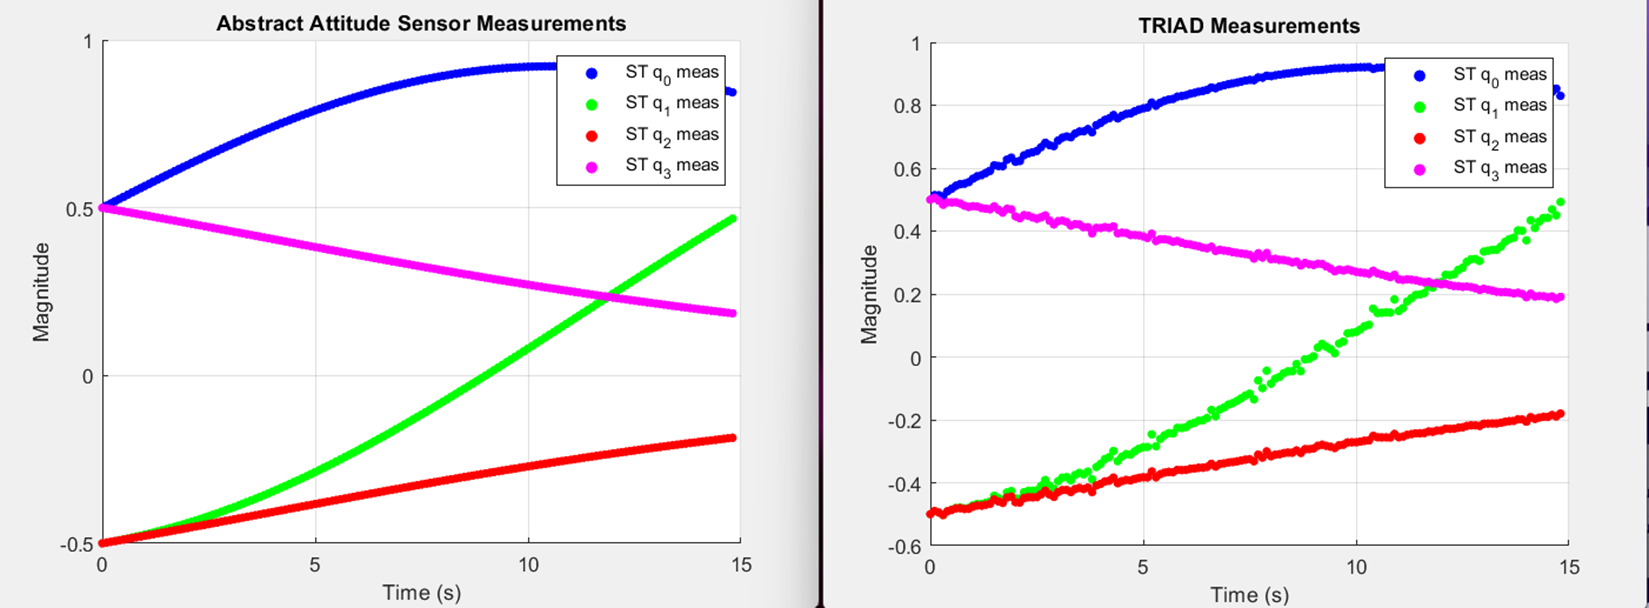
\includegraphics[width=1\textwidth]{figures/modelling/TRIAD.png}
    \caption{}
    \label{fig:CSS}
\end{figure}


\mysubsection{Sensor Comparison}{Sensors Comparison}

\begin{table}[H]
    \caption{Your table caption}
    \footnotesize
    \centering
    \begin{tabular}{lccc}    % <--- define number of columns and alignment
    \toprule
         & Noise Profile & Drift Rate &  Sampling Rate \\
         & & & [Hz] \\
    \midrule
        GPS & 10 m & 3 m & 10 \\
        Gyroscope & 0.05 deg & 1e-3 deg & 50 \\
        Star Tracker & 0.002 deg & - & 1 \\
        CSS & 5 deg & - & 2 \\
        Magnetometer & 10 deg & - & 2 \\
    \bottomrule
    \end{tabular}
    \label{tab:my_label}
\end{table}

\mysection{Conclusion}{Conclusion}
\label{sec:modconclusion}